\section{Limits} \label{S:10.1.Limits}

\vspace*{-14 pt}
\framebox{\hspace*{3 pt}
\parbox{6.25 in}{\begin{goals}
  \item What do we mean by the limit of a function $f$ of two
    variables at a point $(a,b)$?  
  \item What techniques can we use to show that a function of two
    variables does not have a limit at a point $(a,b)$? 
  \item What does it mean for a function $f$ of two variables to be
    continuous at a point $(a,b)$? 
\end{goals}} \hspace*{3 pt}}

\subsection*{Introduction}

In this section, we will study limits of
  functions of several variables, with a focus on limits of functions
  of two variables.   In single variable calculus, we studied the notion of limit, which turned out to be a critical
concept that formed the basis for the derivative and the definite
integral. In this section we will begin to understand how the concept
of limit for functions of two variables is similar to what we
encountered for functions of a single variable.
The limit will again be the fundamental
idea in multivariable calculus, and we will use this notion of the limit
of a function of several variables to define the important concept of
differentiability later in this chapter.  We have already seen its use in the derivatives of vector-valued functions in Section~\ref{S:9.7.Vector_Valued_Functions_Derivatives}.
  
  Let's begin by reviewing what we mean by the
  limit of a function of one variable.  We say that a function $f$ has a limit $L$ as
  $x$ approaches $a$ provided that we can make the values $f(x)$ as close to $L$ as we like
  by taking $x$ sufficiently close (but not equal) to $a$.  We denote this behavior by writing
  $$\lim_{x\to a}f(x) = L.$$

\begin{pa} \label{PA:10.1} 
We investigate the limits of several different functions by working with tables and graphs.
\ba
\item Consider the function $f$ defined by 
  $$
  f(x) = 3-x.
  $$
  Complete the following table of values.
  \begin{center}
    \begin{tabular}{|r|c|}
      \hline      
      $x$ & $f(x)$ \\
      \hhline{|=|=|}
      $-0.2$ & \hspace*{1in} \\
      \hline
      $-0.1$ & \hspace*{1in} \\
      \hline
      0.0 & \hspace*{1in} \\
      \hline
      0.1 & \hspace*{1in} \\
      \hline
      0.2 & \hspace*{1in} \\
      \hline
    \end{tabular}
  \end{center}
  What does the table suggest regarding $\lim_{x\to 0}f(x)$?

\item Explain how your results in (a) are reflected in Figure
  \ref{F:10.1.activity.1}. 

  \begin{figure}[ht]
    \begin{center}
      \scalebox{0.8}{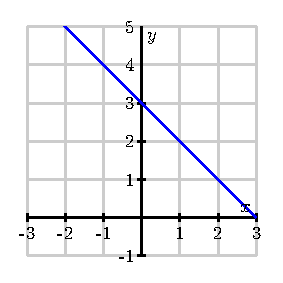
\includegraphics{figures/fig_10_1_activity_3.eps}}
      \caption{The graph of $f(x) = 3-x$.}
      \label{F:10.1.activity.1}
    \end{center}
  \end{figure}
      
      
\item Next, consider $$g(x) = \frac{x}{|x|}.$$
Complete the following table of values near $x = 0$, the point at which $g$ is not defined.
  \begin{center}
    \begin{tabular}{|r|c|}
      \hline      
      $x$ & $g(x)$ \\
      \hhline{|=|=|}
      $-0.1$ & \hspace*{1in} \\
      \hline
      $-0.01$ & \hspace*{1in} \\
      \hline
      $-0.001$ & \hspace*{1in} \\
      \hline
      0.001 & \hspace*{1in} \\
      \hline
       0.01 & \hspace*{1in} \\
      \hline
      0.1 & \hspace*{1in} \\
      \hline
    \end{tabular}
  \end{center}
  What does this suggest about $\lim_{x\to 0}g(x)$?

\item Explain how your results in (c) are reflected in Figure
  \ref{F:10.1.activity.2}. 

  \begin{figure}[ht]
    \begin{center}
      \scalebox{0.8}{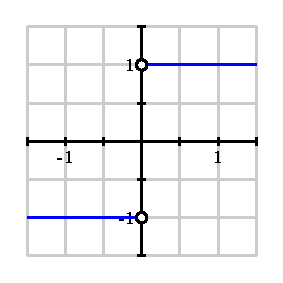
\includegraphics{figures/fig_10_1_activity_2.eps}}
      \caption{The graph of $g(x) = \frac{x}{|x|}$.}
      \label{F:10.1.activity.2}
    \end{center}
  \end{figure}
      
\item Now, let's examine a function of two variables.  Let  
  $$
  f(x,y) = 3 - x - 2y
  $$
  and complete the following table of values.

  \begin{center}
    \begin{tabular}{|r||c|c|c|c|c|}
      \hline
      $x\backslash y$ &$-1$ & $-0.1$ & 0 & 0.1 & 1 \\
      \hhline{|=|=|=|=|=|=|}
      $-1$ & \hspace*{0.5in} & \hspace*{0.5in} & \hspace*{0.5in}  & \hspace*{0.5in} & \hspace*{0.5in} \\
      \hline
      $-0.1$ & & & & & \\
      \hline
      0 & & & & & \\
      \hline
      0.1 & & & & & \\
      \hline
      1 & & & & & \\
      \hline
    \end{tabular}
  \end{center}
  What does the table suggest about $\lim_{(x,y)\to(0,0)} f(x,y)$?

\item Explain how your results in (e) are reflected in Figure
  \ref{F:10.1.activity.4}. Compare this limit to the limit in part (a). How are the limits similar and how are they different?

  \begin{figure}[ht]
    \begin{center}
      \scalebox{0.8}{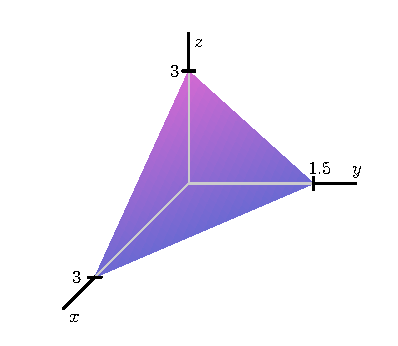
\includegraphics{figures/fig_10_1_limit_contin.eps}}
      \hspace*{0.5in}
      \scalebox{0.8}{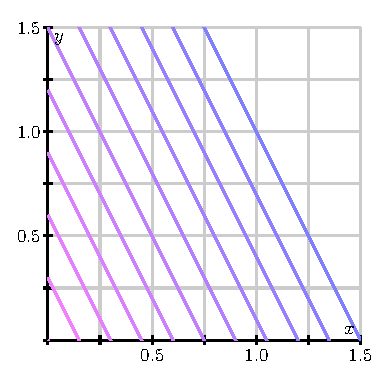
\includegraphics{figures/fig_10_1_cont_contour.eps}}
    \end{center}
      \caption{At left, the graph of $f(x,y) = 3 - x - 2y$; at right, its contour plot.}
      \label{F:10.1.activity.4}
  \end{figure}
      
\item Finally,
  consider
  $$
  g(x,y) = \frac{2xy}{x^2+y^2},
  $$
  which is not defined at $(0,0)$, and complete the following table of values of $g(x,y)$.

  \begin{center}
    \begin{tabular}{|r||c|c|c|c|c|}
      \hline
      $x\backslash y$ &$-1$ &$-0.1$ & 0 & 0.1 & 1 \\
      \hhline{|=|=|=|=|=|=|}
	 $-1$  & \hspace*{0.5in} & \hspace*{0.5in} & \hspace*{0.5in} & \hspace*{0.5in} & \hspace*{0.5in} \\
      \hline
      $-0.1$ & & & & & \\
      \hline
      0  &  &  & --- & & \\
      \hline
       0.1 & & & & & \\
      \hline
      1  & &  & & &  \\
      \hline
    \end{tabular}
  \end{center}
  What does this suggest about $\lim_{(x,y)\to(0,0)} g(x,y)$?

\item Explain how your results are reflected in Figure
  \ref{F:10.1.activity.5}. Compare this limit to the limit in part (b). How are the results similar and how are they different?

  \begin{figure}[ht]
    \begin{center}
      \scalebox{0.8}{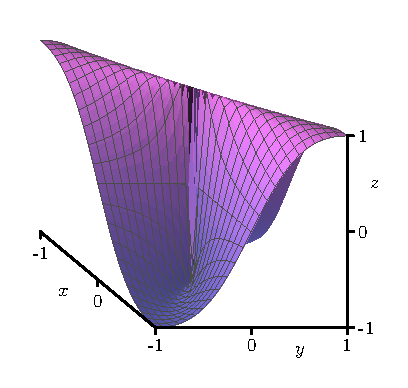
\includegraphics{figures/fig_10_1_limit_disc.eps}}
      \hspace*{0.5in}
      \scalebox{0.8}{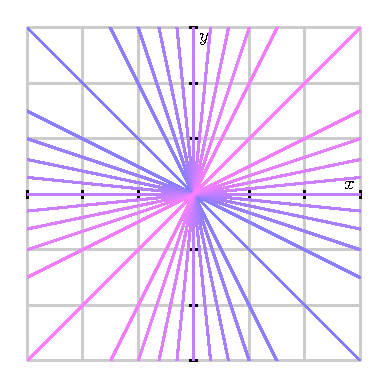
\includegraphics{figures/fig_10_1_limit_contour.eps}}
    \end{center}
      \caption{At left, the graph of $g(x,y) = \frac{2xy}{x^2+y^2}$; at right, its contour plot.}
      \label{F:10.1.activity.5}
  \end{figure}
      
    \ea


\end{pa} 

\begin{activitySolution}
\ba
\item The completed table is below. 
  \begin{center}
    \begin{tabular}{|r|c|}
      \hline      
      $x$ & $f(x)$ \\
      \hhline{|=|=|}
      $-0.2$ & 3.2 \\
      \hline
      $-0.1$ & 3.1 \\
      \hline
      0.0 & 3.0 \\
      \hline
      0.1 & 2.9 \\
      \hline
      0.2 & 2.8 \\
      \hline
    \end{tabular}
  \end{center}
  The table suggests that the values of $f$ get as close to 3 as we want by letting $x$ get as close to 0 as we need. We conclude that 
$\lim_{x\to 0}f(x) = 3$.

\item The graph shows that the points $(x,f(x))$ get as close as we want to the point $(0,3)$ as we let $x$ get as close to 0 as we need. 
      
\item The complete table of values is shown below.
  \begin{center}
    \begin{tabular}{|r|c|}
      \hline      
      $x$ & $g(x)$ \\
      \hhline{|=|=|}
      $-0.1$ & $-1$ \\
      \hline 
      $-0.01$ & $-1$ \\
      \hline
      $-0.001$ & $-1$ \\
      \hline
      0.001 & 1 \\
      \hline
       0.01 & 1 \\
      \hline
      0.1 & 1 \\
      \hline
    \end{tabular}
  \end{center}
  This table suggests that no matter how close we take $x$ to 0, the values of $g(x)$ for $x < 0$ and the values of $g(x)$ for $x > 0$ never get closer than 2. This implies that $\lim_{x\to 0}g(x)$ does not exist. 

\item We can see in the figure that the graph of $g$ makes a jump from $-1$ to $1$ as $x$ changes from negative to positive. This jump discontinuity shows that $g$ does not have a limit at $0$. 
      
\item The complete table of values is below.   

  \begin{center}
    \begin{tabular}{|r||c|c|c|c|c|}
      \hline
      $x\backslash y$ &$-1$ & $-0.1$ & 0 & 0.1 & 1 \\
      \hhline{|=|=|=|=|=|=|}
      $-1$ 	&5 	&4.2 	&4		&3.8 &2 \\
      \hline
      $-0.1$ &5.1 	&3.3 	&3.1 	&2.9 &1.1 \\
      \hline
      0 		&5 	&3.2 	&3 	&2.8 &1 \\
      \hline
      0.1 		&4.9 	&3.1	&2.9 	&2.7 &0.9 \\
      \hline
      1 		&4 	&2.2 	&2 	&1.8 &0 \\
      \hline
    \end{tabular}
  \end{center}
  The values of $f(x,y)$ appear to be approaching 3 as $x$ and $y$ both approach $0$. This suggests that $\lim_{(x,y)\to(0,0)} f(x,y) = 3$.

\item The graph of the surface for $f$ seems to show that the values of $f(x,y)$ approach $3$ as closely as we like as $x$ and $y$ both approach 0. Both $f(x,y) = 3-x-2y$ and $f(x) = 3-x$ are linear functions, so both are continuous everywhere. However, there are only 2 ways as single variable $x$ can approach 0 (from above and from below), while there are many ways that a point $(x,y)$ can approach $(0,0)$. 
      
\item The complete table of values for $g(x,y)$ to three decimal places is below.

  \begin{center}
    \begin{tabular}{|r||c|c|c|c|c|}
      \hline
      $x\backslash y$ &$-1$ &$-0.1$ & 0 & 0.1 & 1 \\
      \hhline{|=|=|=|=|=|=|}
	 $-1$  & 1 & 0.198 & 0 & $-0.198$ & $-1$ \\
      \hline
      $-0.1$ &0.198 &1 &0 &$-1$ &$-0.198$ \\
      \hline
      0  &0  &0  & --- &0 &0 \\
      \hline
       $0.1$ &$-0.198$ &$-1$ &0 &$1$ &$0.198$ \\
      \hline
      $-1$  & $-1$ & $-0.198$ & 0 & $0.198$ & $1$ \\
      \hline
    \end{tabular}
  \end{center}
  The values of $g(x,y)$ are all 0 if $x=0$ or $y=0$. This seems to imply that $g$ has a limit of $0$ at $(0,0)$. However, if $x=y$ we have $g(x,x) = 1$. So the values of $g(x,y)$ do not all get close to the same number as $(x,y)$ approaches $(0,0)$. We conclude that $\lim_{(x,y)\to(0,0)} g(x,y)$ does not exist. 

\item The graph of the surface for $g(x,y) = \frac{2xy}{x^2+y^2}$ seems to show the jump from the values of 0 when $x=0$ or $y=0$ and 1 when $x=y$. This is similar to the graph of $g(x) = \frac{x}{|x|}$ in that there is a jump discontinuity. While $g(x) = \frac{x}{|x|}$ has different one-sided limits at $(0,0)$, it looks like $g(x,y) = \frac{2xy}{x^2+y^2}$ has different limits as $(x,y)$ approaches $(0,0)$ along different paths. 


      
    \ea


\end{activitySolution}

\afterpa 

\subsection*{Limits of Functions of Two Variables}

In Preview Activity \ref{PA:10.1}, we recalled the notion of limit
from single variable calculus and saw that a similar concept applies
to functions of two variables.
Though we will focus on functions of two variables, for the sake of
discussion, all the ideas we establish here are valid for functions of
any number of variables. In a natural followup to our work in Preview Activity \ref{PA:10.1},
we now formally define what it means for a function of two variables to have a
limit at a point.

\vspace*{5pt}
\nin \framebox{\hspace*{3 pt}
  \parbox{6.25 in}{
    \begin{definition} Given a function $f = f(x,y)$, we say that $f$
      {\em has limit $L$ as $(x,y)$ approaches $(a,b)$} provided that we can make
      $f(x,y)$ as close to $L$ as we like by taking $(x,y)$
      sufficiently close (but not equal) to $(a,b)$.  We write 
      $$
      \lim_{(x,y)\to(a,b)} f(x,y) = L.
      $$
    \end{definition}
} \hspace*{3 pt}}
\vspace*{5pt}

To investigate the limit of a single variable function, $\lim_{x\to
  a}f(x)$, we often consider the behavior of $f$ as $x$ approaches
$a$ from the right and from the left.  Similarly, we may investigate
limits of two-variable functions, $\lim_{(x,y)\to(a,b)} f(x,y)$ by
considering the behavior of $f$ as $(x,y)$ approaches $(a,b)$ from
various directions.  This situation is more complicated because there
are infinitely many ways in which $(x,y)$ may approach $(a,b)$.  In the next activity, we
see how it is important to consider a variety of those paths in investigating whether or not a limit exists.

\begin{activity} \label{A:10.1.1} Consider the function $f$, defined by
  $$
  f(x,y) = \frac{y}{\sqrt{x^2+y^2}},
  $$ 
  whose graph is shown below in
  Figure \ref{F:10.1.disc.2}

  \begin{figure}[ht]
    \begin{center}
      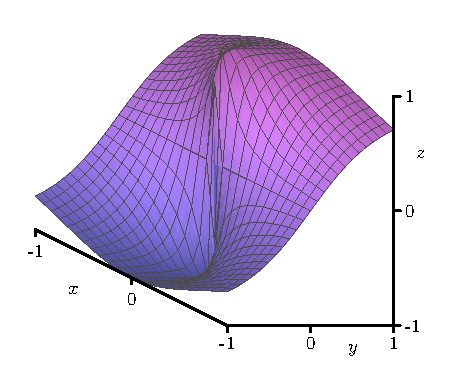
\includegraphics{figures/fig_10_1_disc_2.eps}
      \caption{The graph of $f(x,y) = \frac{y}{\sqrt{x^2+y^2}}$.}
      \label{F:10.1.disc.2}
    \end{center}
  \end{figure}

      
  \ba
\item Is $f$ defined at the point $(0,0)$?  What, if anything, does
  this say about whether $f$ has a limit at the point $(0,0)$? 

\item Values of $f$ (to three decimal places) at several points close to
  $(0,0)$ are shown in the table below. 
  \begin{center}
    \begin{tabular}{|r||c|c|c|c|c|}
      \hline
      $x\backslash y$ & -1 & -0.1 & 0 & 0.1 & 1 \\       \hhline{|=|=|=|=|=|=|}
      $-1$ & $-0.707$ & --- & 0 & ---  & $0.707$ \\       \hline
      $-0.1$ & --- & $-0.707$ & 0 & $0.707$ &  --- \\       \hline
      0 &$-1$ &$-1$ &--- &1 &1 \\       \hline
      0.1 & --- &$-0.707$ &0 &$0.707$ & --- \\       \hline
      1 &$-0.707$ &--- &0 &--- & $0.707$\\       \hline
    \end{tabular}
  \end{center}
%   \begin{center}
%    \begin{tabular}{|c||c|c|c|c|c|}
%      \hline
%      $x\backslash y$ & -1 & -0.1 & 0 & 0.1 & 1 \\
%      \hhline{|=|=|=|=|=|=|}
%      $-1$ & \hspace*{0.5in} & --- & \hspace*{0.5in} & ---
%      & \hspace*{0.5in} \\ 
%      \hline
%      $-0.1$ & --- & \hspace*{0.5in} & & \hspace*{0.5in} &  --- \\
%      \hline
%      0 & & &--- & & \\
%      \hline
%      0.1 & --- & & & & --- \\
%      \hline
%      1 & &--- & &--- & \\
%      \hline
%    \end{tabular}
%  \end{center}
  
  Based on these calculations, state whether $f$ has a limit at
  $(0,0)$ and give an argument supporting your statement. (Hint: The blank spaces in the table are there to help you see the patterns.)
	
\item Now let's consider what happens if we restrict our attention to
  the $x$-axis;  that is, consider what happens when $y = 0$.  
  What is the behavior of $f(x,0)$ as $x \to 0$?  If we approach
  $(0,0)$ by moving along the $x$-axis, what value do we find as the
  limit?  

\item What is the behavior of $f$ along the line $y=x$ when $x> 0$;  that
  is, what is the value of $f(x,x)$ when $x>0$?  If we approach $(0,0)$ by moving
  along the line $y=x$ in the first quadrant (thus considering $f(x,x)$ as $x \to 0$, what value do we find as the limit?

\item In general, if $\lim_{(x,y)\to(0,0)}f(x,y) = L$, then $f(x,y)$ approaches
  $L$ as $(x,y)$ approaches $(0,0)$, regardless of the path we take in letting $(x,y) \to (0,0)$.   Explain what the last two parts
  of this activity imply about the existence of $\lim_{(x,y)\to(0,0)} f(x,y)$.

\item Shown below in Figure \ref{F:10.1.limit_contour_2} is a set of
  contour lines of the function $f$.  What is the behavior of
  $f(x,y)$ as $(x,y)$ approaches $(0,0)$ along any straight line?  
  How does this observation reinforce your conclusion about the
  existence of $\lim_{(x,y)\to(0,0)}f(x,y)$ from the previous part of
  this activity? (Hint: Use the fact that a non-vertical line has equation $y=mx$ for some constant $m$.)

  \begin{figure}[ht]
    \begin{center}
      
\includegraphics{figures/fig_10_1_limit_contour_2.eps}
      \caption{Contour lines of $f(x,y) = \frac{y}{\sqrt{x^2+y^2}}$.}
      \label{F:10.1.limit_contour_2}
    \end{center}
  \end{figure}

	
	
	\ea
\end{activity}

\begin{activitySolution}
\ba
\item Since the denominator is 0 when $(x,y) = (0,0)$, the function $f$ is not defined at the origin. However, a function can have a limit at a point where it is undefined, so this information does not determine if $f$ has a limit at $(0,0)$ or not.
\item It looks as though the values of $f$ are approaching different numbers (e.g., $-1$, $-0.707$, $0.707$, $1$) as $(x,y)$ nears $(0,0)$. The function $f$ will have a limit at the point $(0,0)$ if all of the values of the function become arbitrarily close to one fixed number as $(x,y)$ gets as close to $(0,0)$ as we want. Since the values of $f$ do not approach a single fixed number as $(x,y)$ gets close to $(0,0)$, we should conclude that $f$ does not have a limit at $(0,0)$.   
\item When $y=0$ we have $f(x,y) = f(x,0) = 0$ as indicated in the table. So $\lim_{x \to 0} f(x,0) = 0$. 
\item When $x > 0$ we have $f(x,y) = f(x,x) = \frac{x}{\sqrt{2x^2}} = \frac{1}{\sqrt{2}}$. So  $\lim_{x \to 0} f(x,x) = \frac{1}{\sqrt{2}} \approx 0.707$ as illustrated in the table.
\item The fact that $f(x,y)$ gets arbitrarily close to $0$ as $(x,0)$ gets as close to $(0,0)$ as we want and the fact that $f(x,y)$ gets arbitrarily close to $\frac{1}{\sqrt{2}}$ as $(x,x)$ gets as close to $(0,0)$ as we want shows that there is no fixed number $L$ that all of the values of $f(x,y)$ approach as $(x,y)$ gets close to $(0,0)$. So $f$ does not have a limit at $(0,0)$. 
\item When $y=mx$ we have $f(x,y) = f(x,mx) = \frac{mx}{(1+m^2)x^2}$. If $x>0$, then $f(x,mx) = \frac{m}{1+m^2}$ and if $x < 0$, then $f(x,mx) = -\frac{m}{1+m^2}$. In either case, the values $f(x,mx)$ do not all approach the same number $L$ as $x$ gets arbitrarily close to $0$. In other words, $f$ has different limits along different paths that contain the origin. 
\ea
\end{activitySolution}

\aftera



As we have seen in Activity \ref{A:10.1.1}, if we approach $(a,b)$
along two different paths and find that $f(x,y)$ has two different
limits, we can conclude that $\lim_{(x,y)\to(a,b)}f(x,y)$ does not
exist.  This is similar
to the one-variable example $f(x)=x/|x|$ as shown in
\ref{F:10.1.one.variable}; 
$\lim_{x\to0}f(x)$ does not exist because we see different limits as
$x$ approaches 0 from the left and the right.

  \begin{figure}[ht]
    \begin{center}
      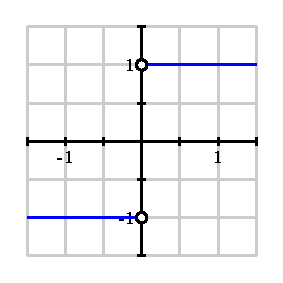
\includegraphics{figures/fig_10_1_activity_2.eps}
      \caption{The graph of $g(x) = \frac{x}{|x|}$.}
      \label{F:10.1.one.variable}
    \end{center}
  \end{figure}

As a general rule, we have 

\vspace*{5pt}
\nin 
\framebox{
  \hspace*{3 pt}
  \parbox{6.25 in}{ 
    If $f(x,y)$ has two different limits as $(x,y)$ approaches $(a,b)$
    along two different paths, then $\lim_{(x,y)\to(a,b)}f(x,y)$ does
    not exist.
  }
  \hspace*{3 pt}
} \vspace*{5pt}

As the next activity shows, studying the limit of a two-variable function
$f(x,y)$ by considering the behavior of $f$ along various paths can require subtle insights. 

\begin{activity} \label{A:10.1.2}  Let's consider the function $g$ defined by 
  $$g(x,y) = \frac{x^2y}{x^4 + y^2}$$
  and investigate the limit $\lim_{(x,y)\to(0,0)}g(x,y)$.

  \ba
\item What is the behavior of $g$ on the $x$-axis?  That is, what is
  $g(x,0)$ and what is the limit of $g$ as $(x,y)$ approaches $(0,0)$
  along the $x$-axis?

\item What is the behavior of $g$ on the $y$-axis?  That is, what is
  $g(0,y)$ and what is the limit of $g$ as $(x,y)$ approaches $(0,0)$
  along the $y$-axis?

\item What is the behavior of $g$ on the line $y=mx$?  That is, what
  is $g(x,mx)$ and what is the limit of $g$ as $(x,y)$ approaches $(0,0)$
  along the line $y=mx$?

\item Based on what you have seen so far, do you think
  $\lim_{(x,y)\to(0,0)}g(x,y)$ exists?  If so, what do you think its
    value is?

\item Now consider the behavior of $g$ on the parabola $y=x^2$?  What
  is $g(x,x^2)$ and what is the limit of $g$ as $(x,y)$ approaches
  $(0,0)$ along this parabola?

\item State whether the limit $\lim_{(x,y)\to(0,0)} g(x,y)$ exists or
  not and provide a justification of your statement.



  \ea


\end{activity}

\begin{activitySolution}
\ba
\item Along the $x$-axis we have $g(x,0) = 0$, so $\lim_{(x,y) \to (0,0)} g(x,0) = 0$. 
\item Along the $y$-axis we have $g(0,y) = 0$, so $\lim_{(x,y) \to (0,0)} g(0,y) = 0$.
\item Along the line $y=mx$ we have $g(x,mx) = \frac{mx^3}{x^4 + m^2x^2} = \frac{mx}{x^2+m^2}$. So as $x$ goes to $0$ we have $\lim_{(x,y) \to (0,0)} g(x,mx) = 0$.
\item Based on the previous information, we might be tempted to say that $g$ has a limit of $0$ at $(0,0)$.  
\item Along the parabola $y=x^2$ we have $g(x,x^2) = \frac{x^4}{2x^4} = \frac{1}{2}$. So as $x$ goes to $0$ we have $\lim_{(x,y) \to (0,0)} g(x,x^2) = 0.5$.
\item Since $g$ has different limits along different paths that contain $(0,0)$, we conclude that $\lim_{(x,y) \to (0,0)} g(x,y)$ does not exist. 
\ea
\end{activitySolution}

\aftera


This activity shows that we need to be careful when studying the limit
of a two-variable functions by considering its behavior along
different paths.  If we find two
different paths that result in two different limits, then we may
conclude that the limit does not exist.  However, we can never
conclude that the limit of a function exists only by considering its
behavior along different paths.

Generally speaking, concluding that a limit
$\lim_{(x,y)\to(a,b)}f(x,y)$ exists requires a more careful
argument.  For example, let's consider the function
$$
f(x,y) = \frac{x^2y^2}{x^2+y^2}
$$
and ask whether $\lim_{(x,y)\to(0,0)}f(x,y)$ exists.

Note that if either $x$ or $y$ is 0, then $f(x,y) = 0$. Therefore, if
$f$ has a limit at $(0,0)$, it must be 0.  We will therefore argue
that
$$
\lim_{(x,y)\to(0,0)}f(x,y) = 0,
$$
by showing that we can make $f(x,y)$ as close to $0$ as we wish by taking $(x,y)$ sufficiently close (but not equal) to $(0,0)$.  In what follows, we view $x$ and $y$ as being real numbers that are close, but not equal, to 0.

Since $0 \leq x^2$, we have 
$$
y^2 \leq x^2+y^2,
$$
which implies that
$$\frac{y^2}{x^2+y^2} \leq 1.$$
Multiplying both sides by $x^2$ and observing that $f(x,y) \ge 0$ for all $(x,y)$ gives
$$
0\leq f(x,y) = \frac{x^2y^2}{x^2+y^2} =
x^2\left(\frac{y^2}{x^2+y^2}\right) \leq x^2.
$$
This shows that we can make $f(x,y)$ as close to $0$ as we like
by taking $x$ sufficiently close to $0$ (for this example, it turns out that we don't even need to worry about making $y$ close to 0).  Therefore,
$$
\lim_{(x,y) \to (0,0)} \frac{x^2y^2}{x^2+y^2} = 0.
$$

In spite of the fact that these two most recent examples 
illustrate some of the complications that arise when studying limits
of two-variable functions, many of the properties that are familiar
from our study of single variable functions hold in precisely the same
way.  For instance, 

\vspace*{5pt}
\nin \framebox{\hspace*{3 pt}
\parbox{6.25 in}{
  \textbf{Properties of Limits.} Let $f(x,y)$ and $g(x,y)$ be
  functions so that $\ds \lim_{(x,y) \to
    (a,b)} f(x,y)$ and $\ds \lim_{(x,y) \to (a,b)} g(x,y)$ both
  exist. Then
\begin{enumerate}
  \item $\ds \lim_{(x,y)\to(a,b)} x = a$ \ \ \ and \ \ \ $\ds \lim_{(x,y)\to(a,b)}
    y = b$.
\item $\ds \lim_{(x,y) \to (a,b)} cf(x,y) = c\left(\lim_{(x,y) \to (a,b)}
  f(x,y)\right)$ for any scalar $c$, 
\item $\ds \lim_{(x,y) \to (a,b)} [f(x,y)\pm g(x,y)] = \lim_{(x,y) \to
    (a,b)} f(x,y) \pm \lim_{(x,y) \to (a,b)} g(x,y)$, 
%\item $\ds \lim_{(x,y) \to (a,b)} [f(x,y)-g(x,y)] = \lim_{(x,y) \to
 %   (a,b)} f(x,y) - \lim_{(x,y) \to (a,b)} g(x,y)$, 
\item $\ds \lim_{(x,y) \to (a,b)} [f(x,y) \cdot g(x,y)] = \left(\lim_{(x,y) \to
    (a,b)} f(x,y)\right) \cdot \left(  \lim_{(x,y) \to (a,b)} g(x,y)\right)$, 
\item $\ds \lim_{(x,y) \to (a,b)} \frac{f(x,y)}{g(x,y)} =
  \frac{\lim_{(x,y) \to (a,b)} f(x,y)}{\lim_{(x,y) \to (a,b)} g(x,y)}$
 \ \ \ if \ \ \ $\ds \lim_{(x,y) \to (a,b)} g(x,y) \neq 0$. 
\end{enumerate}
} \hspace*{3 pt}}
\vspace*{5pt}

We can use these properties and results from single variable calculus
to verify that many limits exist. For example, these properties show
that the function $f$ 
defined by 
$$
f(x,y) = 3x^2y^3 + 2xy^2 - 3x + 1
$$ 
has a limit at every point $(a,b)$ and, moreover, 
$$
\lim_{(x,y)\to(a,b)} f(x,y) = f(a,b).
$$
The reason for this is that polynomial functions of a single variable have limits at every point. 

\subsection*{Continuity}

Recall that a function $f$ of a single variable $x$ is said to be
continuous at 
$x=a$ provided that the following three conditions are satisfied: 
\begin{enumerate}
  \item $f(a)$ exists,
  \item $\lim_{x\to a}f(x)$ exists, and 
  \item $\lim_{x\to a}f(x)=f(a)$.
\end{enumerate}
Using our understanding of limits of multivariable functions, we can
define continuity in the same way. 

\vspace*{5pt}
\nin \framebox{\hspace*{3 pt}
\parbox{6.25 in}{
  \begin{definition} A function $f(x,y)$ 
    is \textbf{continuous}\index{continuity} at the point $(a,
    b)$ provided that
    \begin{enumerate}
    \item $f$ is defined at the point $(a, b)$,
    \item $\ds \lim_{(x,y) \to (a,b)} f(x,y)$ exists, and
    \item $\ds \lim_{(x,y) \to (a,b)} f(x,y) = f(a,b)$.
    \end{enumerate}
  \end{definition}
} \hspace*{3 pt}}
\vspace*{5pt}

For instance, we have seen that the function $f(x,y) = 3x^2y^3 + 2xy^2
- 3x + 1$ is continous at every point.  And just as with single variable functions, continuity has certain
properties that are based on the properties of limits. 

\vspace*{5pt}
\nin \framebox{\hspace*{3 pt}
\parbox{6.25 in}{\textbf{Properties of Continuity.} Let $f$ and
  $g$ be functions of two variables that are continuous at the point $(a,b)$. Then 
  \begin{enumerate}
  \item $cf$ is continuous at $(a,b)$ for any scalar $c$
  \item $f+g$ is continuous at $(a,b)$
  \item $f-g$ is continuous at $(a,b)$
  \item $fg$ is continuous at $(a,b)$
  \item $\frac{f}{g}$ is continuous at $(a,b)$ if $g(a,b) \neq 0$
  \end{enumerate}
} \hspace*{3 pt}}
\vspace*{5pt}

Using these properties, we can apply results from single variable calculus
to decide about continuity of multivariable functions. For example, the coordinate functions $f$ and $g$ defined by $f(x,y) = x$ and $g(x,y) = y$ are continuous at every point. We can then use properties of continuity listed to conclude that every polynomial function in $x$ and $y$ is continuous at every point. For example, $g(x,y)=x^2$ and $h(x,y)=y^3$ are continuous functions, so their product $f(x,y) = x^2y^3$ is a continuous multivariable function. 


\begin{summary}
\item A function $f = f(x,y)$ has a limit $L$ at a point $(a,b)$ provided that we
  can make $f(x,y)$ as close to $L$ as we like by taking $(x,y)$
  sufficiently close (but not equal) to $(a,b)$.  
\item If $(x,y)$ has two different limits as $(x,y)$ approaches
  $(a,b)$ along two different paths, we can conclude that
  $\lim_{(x,y)\to(a,b)}f(x,y)$ does not exist.
\item Properties similar to those for one-variable functions allow us
  to conclude that many limits exist and to evaluate them.
\item A function $f = f(x,y)$ is continuous at a point $(a,b)$ in its
  domain if $f$ has a limit at $(a,b)$ and 
\[f(a,b) = \lim_{(x,y) \to (a,b)} f(x,y).\] 
\end{summary}



\nin \hrulefill

\begin{exercises} 

\item \label{Ez:10.1.1}    Consider the function $f$ defined by $\ds f(x,y) = \frac{xy}{x^2 + y^2 + 1}.$
				
    \ba
   	\item What is the domain of $f$?
	\item Evaluate limit of $f$ at $(0,0)$ along the following paths:  $x = 0$, $y = 0$, $y = x$, and $y = x^2$.
	\item What do you conjecture is the value of $\ds \lim_{(x,y) \to (0,0)} f(x,y)$?
	\item Is $f$ continuous at $(0,0)$?  Why or why not?
	\item Use appropriate technology to sketch both surface and contour plots of $f$ near $(0,0)$.  Write several sentences to say how your plots affirm your findings in (a) - (d).
    \ea

\begin{exerciseSolution}
    \ba
   	\item As a rational function, $f$ is defined everywhere except at the points where the denominator is 0. Since $x^2 + y^2 + 1 \geq 1$ for every $x$ and $y$, the domain of $f$ is all ordered pairs $(x,y)$, or the entire $x$-$y$ plane. 
	\item Along the path $x=0$ we have 
\[\lim_{(x,y) \to (0,0)} f(0,y) = \lim_{y \to 0} \frac{0}{y^2+1} = 0.\]
Along the path $y=0$ we have 
\[\lim_{(x,y) \to (0,0)} f(x,0) = \lim_{x \to 0} \frac{0}{x^2+1} = 0.\]
Along the path $y=x$ we have 
\[\lim_{(x,y) \to (0,0)} f(x,x) = \lim_{x \to 0} \frac{x^2}{2x^2+1} = 0.\]
Along the path $y=x^2$ we have 
\[\lim_{(x,y) \to (0,0)} f(x,x^2) = \lim_{x \to 0} \frac{x^3}{x^4+x^2+1} = 0.\]
	\item The results of the previous part of this problem indicate that $f$ may have a limit at $(0,0)$ and that limit is 0.
	\item If $\lim_{(x,y) \to (0,0)} f(x,y) = 0$, then $\lim_{(x,y) \to (0,0)} f(x,y) = f(0,0)$ and $f$ is continuous at $(0,0)$. 
	\item The surface defined by $f$ has a saddle shape around $(0,0)$ and appears to be in one piece around $(0,0)$, which indicates that $f$ is continuous at $(0,0)$. 
    \ea
\end{exerciseSolution}

\item \label{Ez:10.1.2}    Consider the function $g$ defined by $\ds g(x,y) = \frac{xy}{x^2 + y^2}.$
				
    \ba
   	\item What is the domain of $g$?
	\item Evaluate limit of $g$ at $(0,0)$ along the following paths:  $x = 0$, $y = x$, and $y = 2x$.
	\item What can you now say about the value of $\ds \lim_{(x,y) \to (0,0)} g(x,y)$?
	\item Is $g$ continuous at $(0,0)$?  Why or why not?
	\item Use appropriate technology to sketch both surface and contour plots of $g$ near $(0,0)$.  Write several sentences to say how your plots affirm your findings in (a) - (d).
    \ea

\begin{exerciseSolution}
    \ba
   	\item As a rational function, $g$ is defined everywhere except at the points where the denominator is 0. Since $x^2 + y^2  = 0$ only when $x=y=0$, the domain of $g$ is all ordered pairs $(x,y)$ not equal to $(0,0)$, or the $x$-$y$ plane with the origin removed. 
	\item Along the path $x=0$ we have 
\[\lim_{(x,y) \to (0,0)} g(0,y) = \lim_{y \to 0} \frac{0}{y^2} = 0.\]
Along the path $y=x$ we have 
\[\lim_{(x,y) \to (0,0)} g(x,x) = \lim_{x \to 0} \frac{x^2}{2x^2} = \frac{1}{2}.\]
Along the path $y=2x$ we have 
\[\lim_{(x,y) \to (0,0)} f(x,2x) = \lim_{x \to 0} \frac{2x^2}{5x^2} = \frac{2}{5}.\]
	\item The results of the previous part of this problem show that $g$ has different limits at $(0,0)$ along different paths, so $g$ does not have a limit at $(0,0)$.
	\item Either of the conditions: $g$ is not defined at $(0,0)$, $g$ does not have a limit at $(0,0)$, show that $g$ is not continuous at $(0,0)$. 
	\item The surface defined by $g$ appears to have a tear in it at the origin, indicating that $g$ is not continuous at $(0,0)$. 
    \ea
\end{exerciseSolution}


\item \label{Ez:10.1.3}  For each of the following prompts, provide an example of a function of two variables with the desired properties (with justification), or explain why such a function does not exist.
				
    \ba
   	\item A function $p$ that is defined at $(0,0)$, but $\ds \lim_{(x,y) \to (0,0)} p(x,y)$ does not exist.
	\item A function $q$ that does not have a limit at $(0,0)$, but that has the same limiting value along any line $y = mx$ as $x \to 0$.
	\item A function $r$ that is continuous at $(0,0)$, but $\ds \lim_{(x,y) \to (0,0)} r(x,y)$ does not exist.
	\item A function $s$ such that 
	$$\lim_{(x,x) \to (0,0)} s(x,x) = 3 \ \ \ \mbox{and} \ \ \ \lim_{(x,2x) \to (0,0)} s(x,2x) = 6,$$
	for which  $\ds \lim_{(x,y) \to (0,0)} s(x,y)$ exists.
	\item A function $t$ that is not defined at $(1,1)$ but $\ds \lim_{(x,y) \to (1,1)} t(x,y)$ does exist.
    \ea

\begin{exerciseSolution}
    \ba
   	\item Let $p(x,y) = \frac{2x+y}{x+y}$ if $(x,y) \neq (0,0)$ and $p(0,0) = 0$. So $p$ is defined at $(0,0)$ by definition. Note that 
\[\lim_{(x,y) \to (0,0)} p(0,y) = \lim_{y \to 0} \frac{y}{y} = 1\]
but
\[\lim_{(x,y) \to (0,0)} p(x,0) = \lim_{x \to 0} \frac{2x}{x} = 2,\]
so $p$ does not have a limit at $(0,0)$. 
	\item Let $q(x,y) = \frac{x^2y}{x^4+y^2}$as in Activity \ref{A:10.1.2}. Along the line $y=mx$ we have 
\[\lim_{(x,y) \to (0,0)} q(x,mx) = \lim_{x \to 0} \frac{mx^3}{x^2(x^2+m^2)} = \lim_{x \to 0} \frac{mx}{x^2+m^2} = 0,\] 
so $q$ has the same limiting value along any line $y = mx$ as $x \to 0$. However,
\[\lim_{(x,y) \to (0,0)} q(x,x^2) = \lim_{x \to 0} \frac{x^4}{2x^4} = \frac{1}{2},\]
	\item By definition, if $r$ is continuous at $(0,0)$, then $\ds \lim_{(x,y) \to (0,0)} r(x,y)$ exists and is equal to $r(0,0)$. So there is no such function.
	\item The first limit is the same as $\ds \lim_{(x,y) \to (0,0)} s(x,y) = 3$ along the path $y=x$ and the second is $\ds \lim_{(x,y) \to (0,0)} s(x,y) = 6$ along the path $y=2x$. So $s$ has different limits at $(0,0)$ along different paths. Therefore, there is no such function for which $\ds \lim_{(x,y) \to (0,0)} s(x,y)$ exists.
	\item In this section we showed that the function $f$ defined by 
\[f(x,y) = \frac{x^2y^2}{x^2+y^2}\]
is not defined at $(0,0)$ but has a limit at $(0,0)$. We can translate this function to 
\[t(x,y) = \frac{(x-1)^2(y-1)^2}{(x-1)^2+(y-1)^2},\]
that is not defined at $(1,1)$ but for which $\ds \lim_{(x,y) \to (1,1)} t(x,y)$ does exist (and is $0$).
    \ea
\end{exerciseSolution}


\end{exercises}
\afterexercises


\clearpage
